\documentclass{article}
\usepackage{amsmath}
\usepackage{amssymb}
\usepackage{amsfonts}
\usepackage{mathrsfs}
\usepackage{graphicx}
\usepackage{float}
\usepackage[margin=1in]{geometry}
\usepackage{tikz}
\usepackage{pgfplots}
\usetikzlibrary{
    shapes.multipart, 
    arrows.meta, 
    positioning, 
    calc,           % Complex calculations ke liye
    automata,       % State machines (q0 -> q1) ke liye
    trees,          % Probability trees ke liye
    patterns,       % Shading/Hatching ke liye
    quotes          % Label on lines ke liye
}
\tikzset{
    class/.style={
        rectangle split, 
        rectangle split parts=3, 
        draw, 
        align=left, 
        text width=4cm,
        font=\small
    },
    abstract/.style={
        class,
        font=\itshape
    },
    inheritance/.style={
        -{Triangle[open]}, 
        thick
    }
}
% Safety net: Common AI hallucinated commands for UML diagrams
\providecommand{\attribute}[1]{\textit{#1}}
\providecommand{\method}[1]{\texttt{#1}}
\providecommand{\classname}[1]{\textbf{#1}}
\begin{document}

\hrule
\vspace{0.5em}
\noindent \textbf{Question \# 4: CLO-3} \hfill \textbf{Marks: [15] Time: [30 mins]}
\vspace{0.5em}
\hrule
\vspace{1em}

\noindent \textbf{Consider the following Problem Statement:}
Suppose we have an employee record system in which we have different types of employees i.e. trainee employees (on probation) and some of the regular employees (salaried and hourly based). Consider the following design given below in \textit{Figure-1}, it can be observed that
\begin{itemize}
    \item Salaried Employee has a fixed amount of salary.
    \item Hourly Employee gets payment on the basis of the total hours he/she worked in a month.
    \item Trainee Employee gets payment in the form of a commission based on the items he/she sold in a month e.g. 10\$ for one product.
    \item Employee class has an abstract method named earnings (calculating earnings of the employee). All the derived classes have to provide their implementation.
\end{itemize}

\noindent \textbf{Abstract Class}

\begin{figure}[h!]
    \centering
    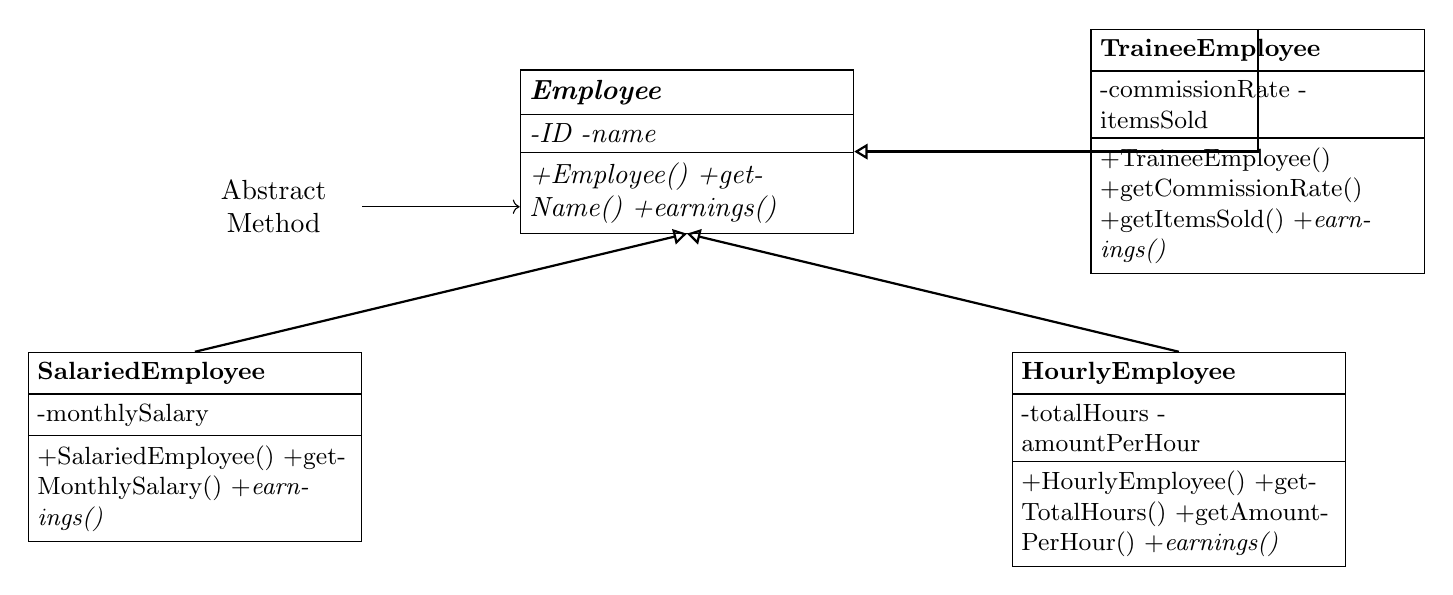
\begin{tikzpicture}
        % Employee (Abstract Class)
        \node [abstract] (employee) {
            \textbf{Employee}
            \nodepart{two}
            -ID
            -name
            \nodepart{three}
            +Employee()
            +getName()
            +\textit{earnings()}
        };

        % TraineeEmployee (Regular Class)
        \node [class, right=3cm of employee] (trainee) {
            \textbf{TraineeEmployee}
            \nodepart{two}
            -commissionRate
            -itemsSold
            \nodepart{three}
            +TraineeEmployee()
            +getCommissionRate()
            +getItemsSold()
            +\textit{earnings()}
        };

        % SalariedEmployee (Regular Class)
        \node [class, below left=1.5cm and 2cm of employee] (salaried) {
            \textbf{SalariedEmployee}
            \nodepart{two}
            -monthlySalary
            \nodepart{three}
            +SalariedEmployee()
            +getMonthlySalary()
            +\textit{earnings()}
        };

        % HourlyEmployee (Regular Class)
        \node [class, below right=1.5cm and 2cm of employee] (hourly) {
            \textbf{HourlyEmployee}
            \nodepart{two}
            -totalHours
            -amountPerHour
            \nodepart{three}
            +HourlyEmployee()
            +getTotalHours()
            +getAmountPerHour()
            +\textit{earnings()}
        };

        % Inheritance arrows
        % TraineeEmployee to Employee
        \draw [inheritance] (trainee.north) |- (employee.east);

        % SalariedEmployee to Employee
        \draw [inheritance] (salaried.north) -- (employee.south);

        % HourlyEmployee to Employee
        \draw [inheritance] (hourly.north) -- (employee.south);

        % Abstract Method note
        \node [left=2cm of employee.west, yshift=-0.7cm, text width=2cm, align=center] (abstract_method_note) {Abstract\\Method};
        \draw [->] (abstract_method_note.east) -- ($(employee.west) + (0,-0.7cm)$);
    \end{tikzpicture}
    \caption{\textit{Figure 1 Class Diagram}}
\end{figure}

Everything seems satisfactory until we think about the life of a trainee employee object. Trainee Employees can become regular employees after the probation period. If we delete the trainee employee object and create a new object of salary or hourly-based employee, then we have to destroy all the previous associations and links of that object as well which is a maintenance nightmare. This is known as object morphing when an object wants to change its behaviour.
\begin{itemize}
    \item Re-Structure the above design to avoid maintenance issues and object morphing. Also, write some justification about your design strategy.
    \item \textbf{Hint:} Use Behavioral Design Patterns.
\end{itemize}

\vspace{1em}
\hrule
\vspace{0.5em}
\noindent \textbf{Question \# 5: CLO-4} \hfill \textbf{Marks: [15] Time: [30 mins]}
\vspace{0.5em}
\hrule
\vspace{1em}

\noindent \textbf{ATM System:}
A local bank intends to install a new automated teller machine (ATM) to allow users (i.e., bank customers) to perform basic financial transactions. ATM users should be able to view their account balance, withdraw cash (i.e., take money out of an account) and deposit funds (i.e., place money into an account). Consider the class diagram in \textit{Figure 2} for your reference:

\end{document}